\documentclass{beamer}
\usepackage[utf8]{inputenc}
\usepackage[]{amsmath}
\usepackage{graphicx}
\usepackage{subcaption} % package pour faire des subfigures
\usepackage{multirow} % package pour multirow/multicolumn
\usepackage{booktabs} % package pour top/mid/bottom rule
\usepackage{tcolorbox} % toujours plus de boites
\usepackage[backend=biber]{biblatex}


\addbibresource{Biblio_dbl_quantum.bib}

%\bibliographystyle{stylename}
%\bibliography{Biblio_dbl_quantum}

\title{Group meeting : Cross-relaxation with NV centers ensemble in diamond}
%\author{Clément Pellet-Mary\\ Laboratoire de physique de l'ENS\\ \textit{ENS, Paris}}
\date\today

\mode<presentation> {\usetheme{Rochester}}

\begin{document}
\begin{frame}
\maketitle
\end{frame}
\begin{frame}
\tableofcontents
\end{frame}
\section{The NV center}
\begin{frame}
\tableofcontents[currentsection]
\end{frame}
\begin{frame}{The Nitrogen Vacancy Center}
\begin{center}
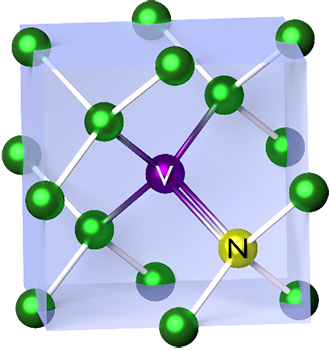
\includegraphics[scale=.4]{Nitrogen-vacancy_center}
\end{center}
\begin{itemize}
\item 0D fluorescent object with ZPL at 638 nm
\item Controllable and readable spin at room temperature (!)
\item Working with 10$^9$ emitters (typ.)
\end{itemize}
\end{frame}
\begin{frame}{NV center : Optical properties}
\centering
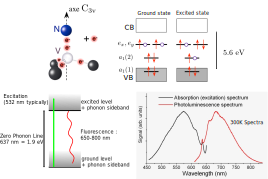
\includegraphics[scale=.4]{slide_NV_optical}
\end{frame}
\begin{frame}{NV center : 8 levels}
\centering
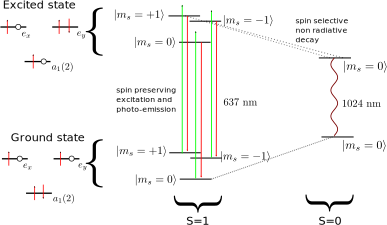
\includegraphics[scale=.3]{NV_8_niveaux}
\end{frame}
\begin{frame}{NV center : 3 levels}
\centering
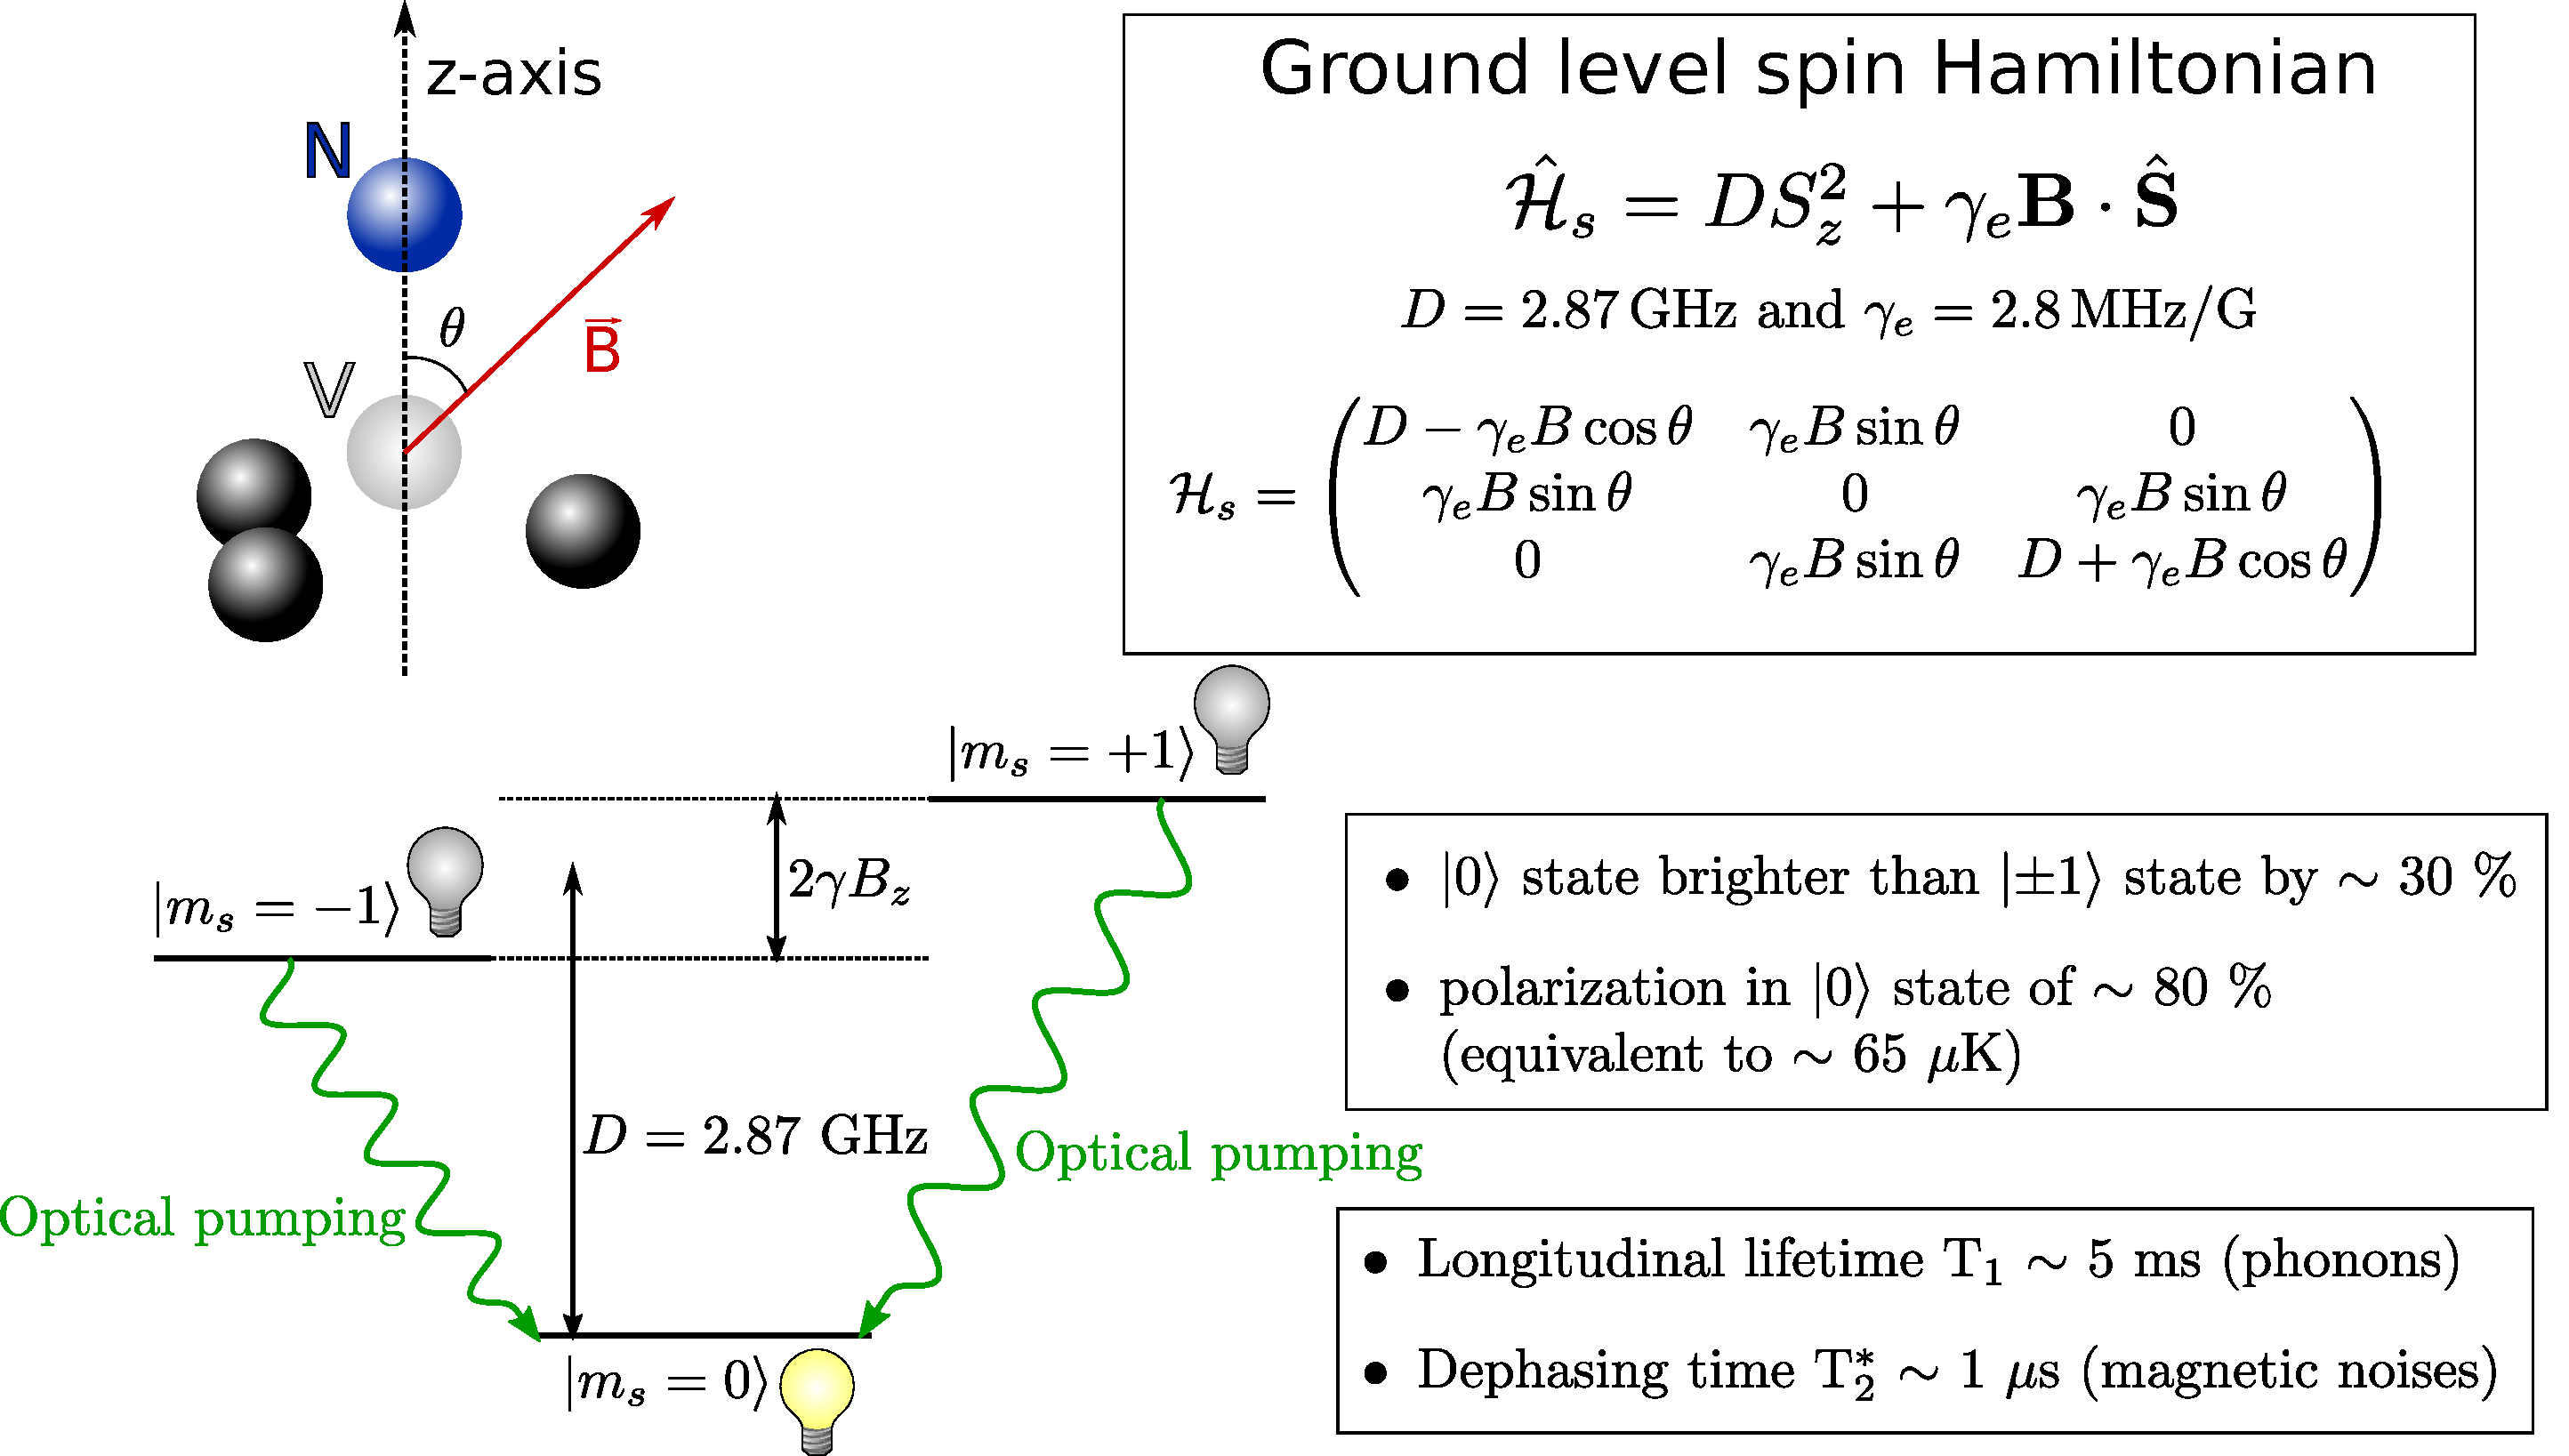
\includegraphics[scale=.23]{slide_3_niveaux}
\end{frame}
\begin{frame}{Spin manipulation}
\centering
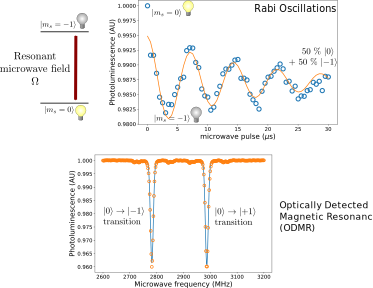
\includegraphics[scale=.25]{slide_rabi_odmr}
\end{frame}
\begin{frame}{Summary : Magnetometry with NV centers}
\centering
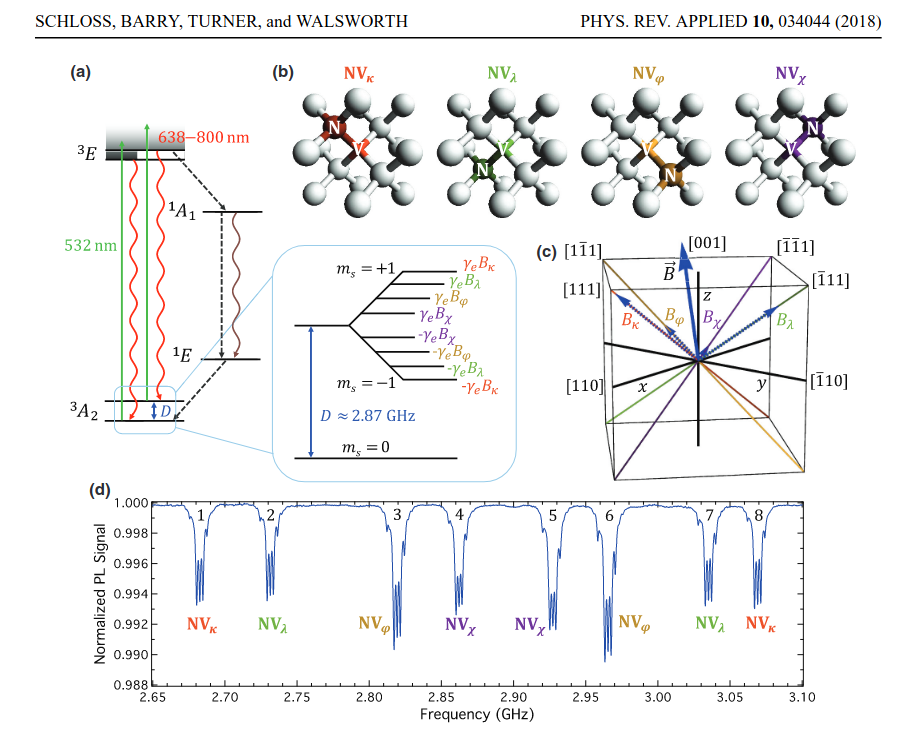
\includegraphics[scale=.4]{ESR_8raies_article}
\end{frame}
\section{Probing dark spins with cross-relaxations}
\begin{frame}
\tableofcontents[currentsection]
\end{frame}
\begin{frame}{Principle of spin cross-relaxation (CR)}
\centering
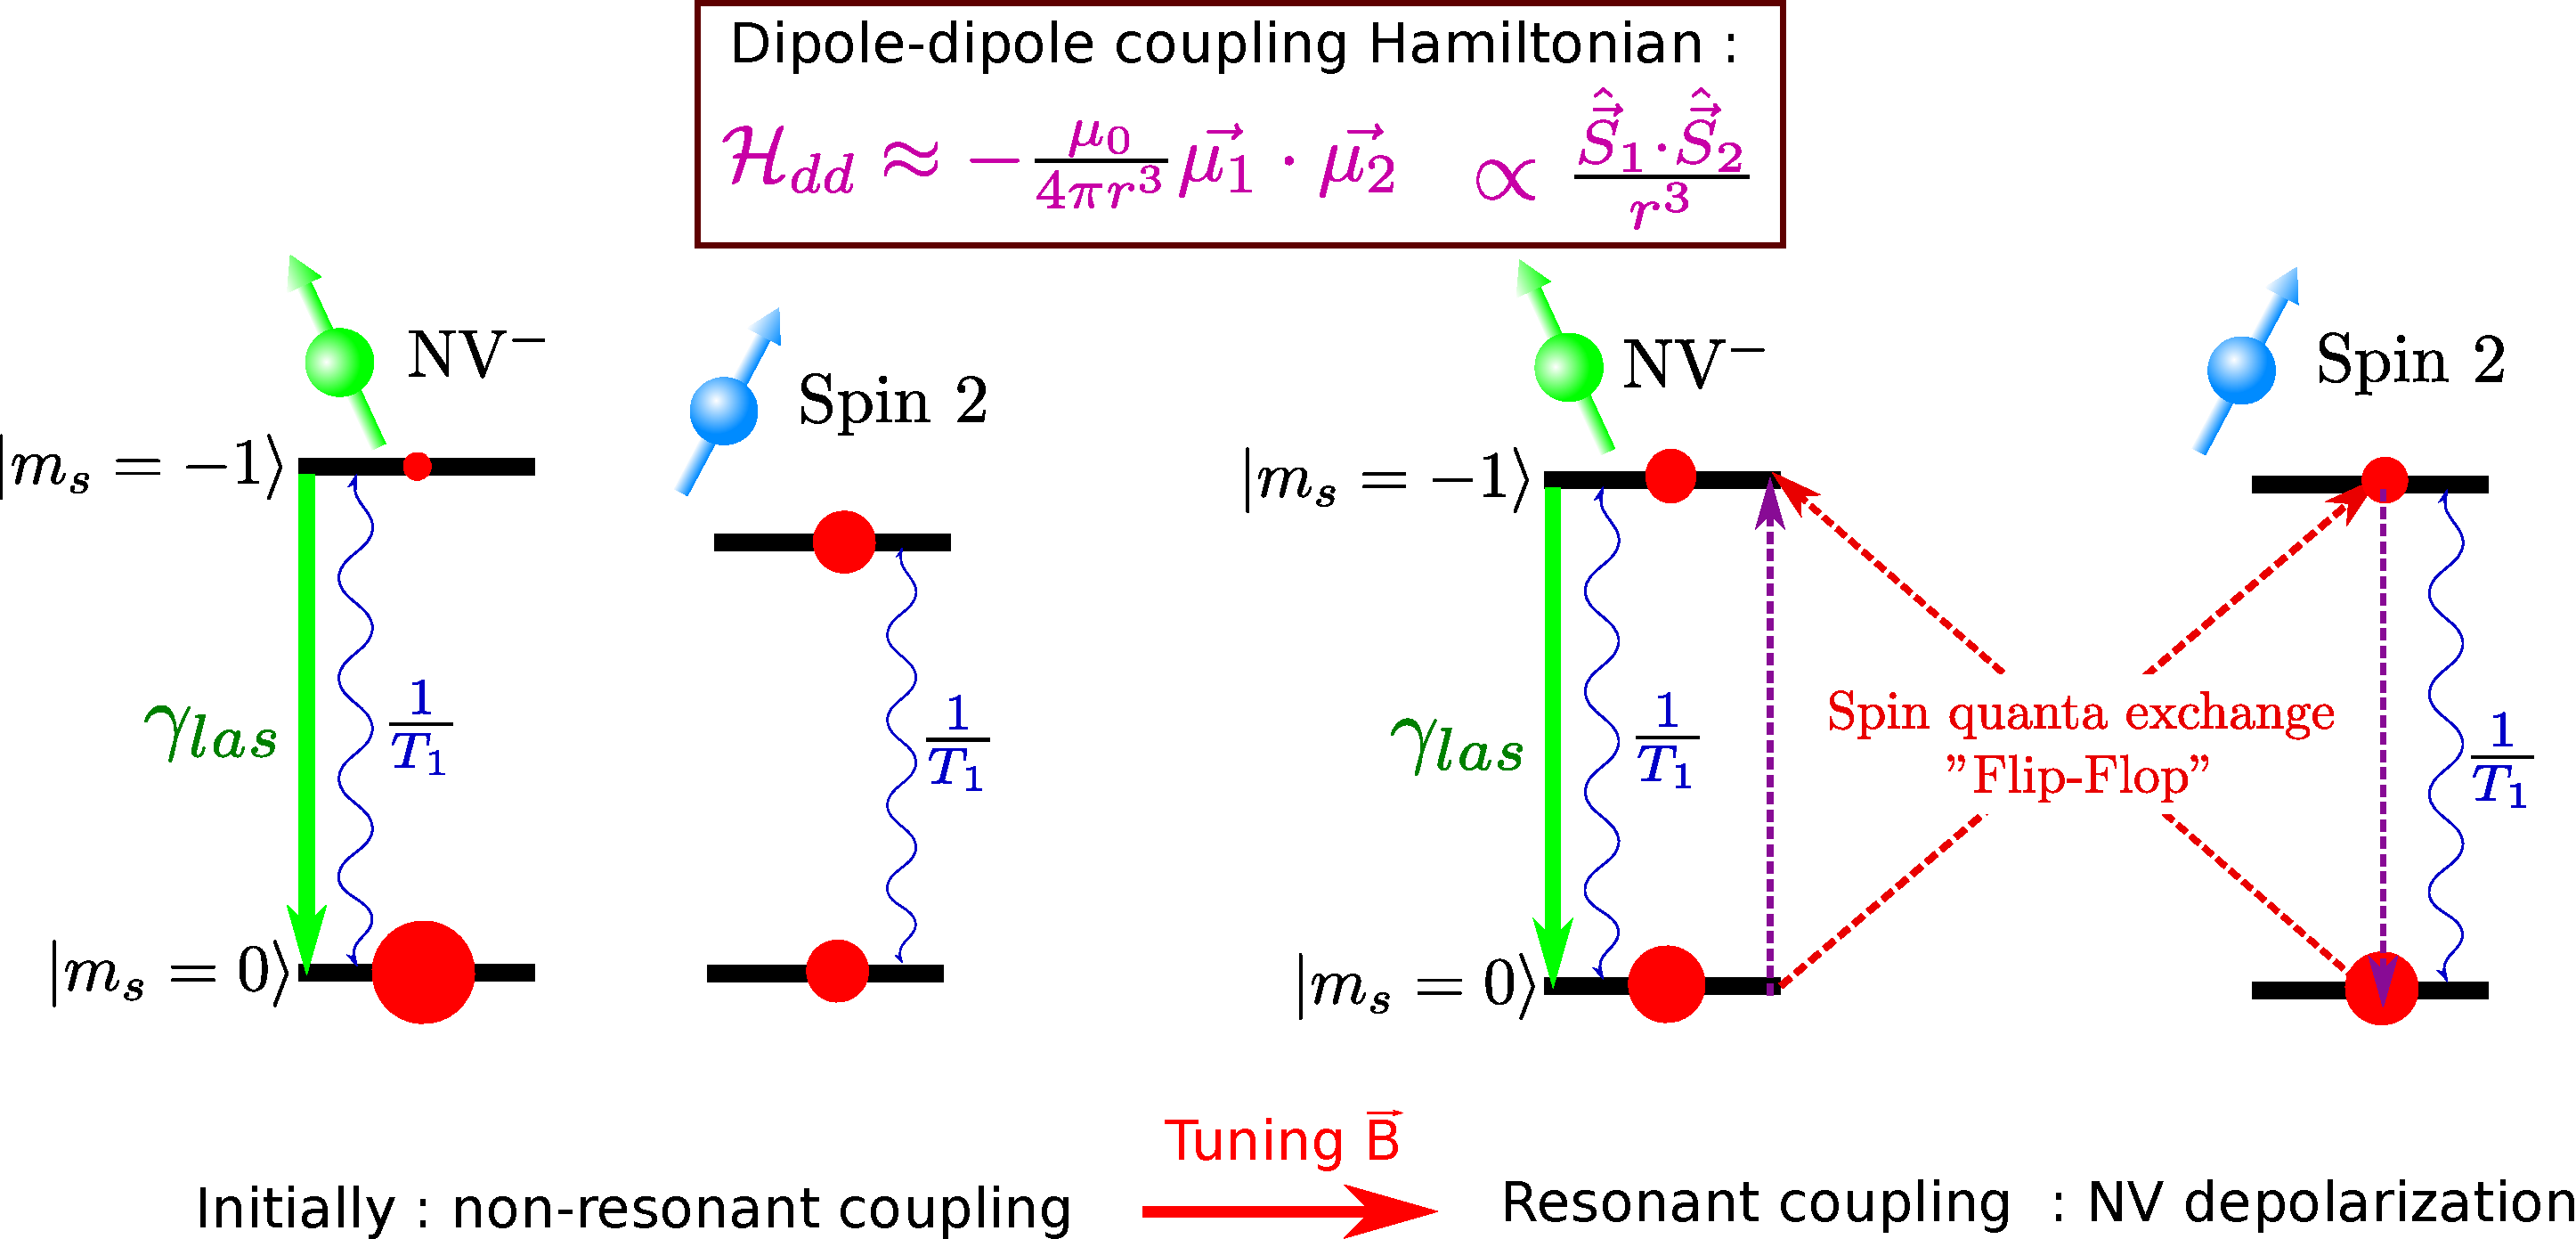
\includegraphics[scale=.23]{Slide_CR}
\end{frame}
\begin{frame}{Detection of dark spins in CVD sample}
\centering
\includegraphics[scale=.35]{Slide_CR_CVD}
\end{frame}
\begin{frame}{Side-note : effect of transverse field on the PL}
\centering
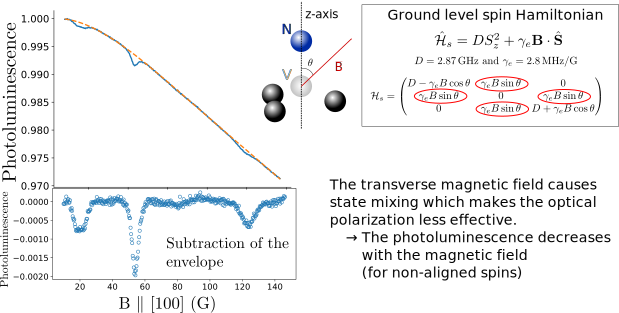
\includegraphics[scale=.18]{slide_champ_transverse}
\end{frame}
\section{NV-NV Cross-relaxation}
\begin{frame}
\tableofcontents[currentsection]
\end{frame}
\begin{frame}{NV-NV Cross-Relaxation}
\centering
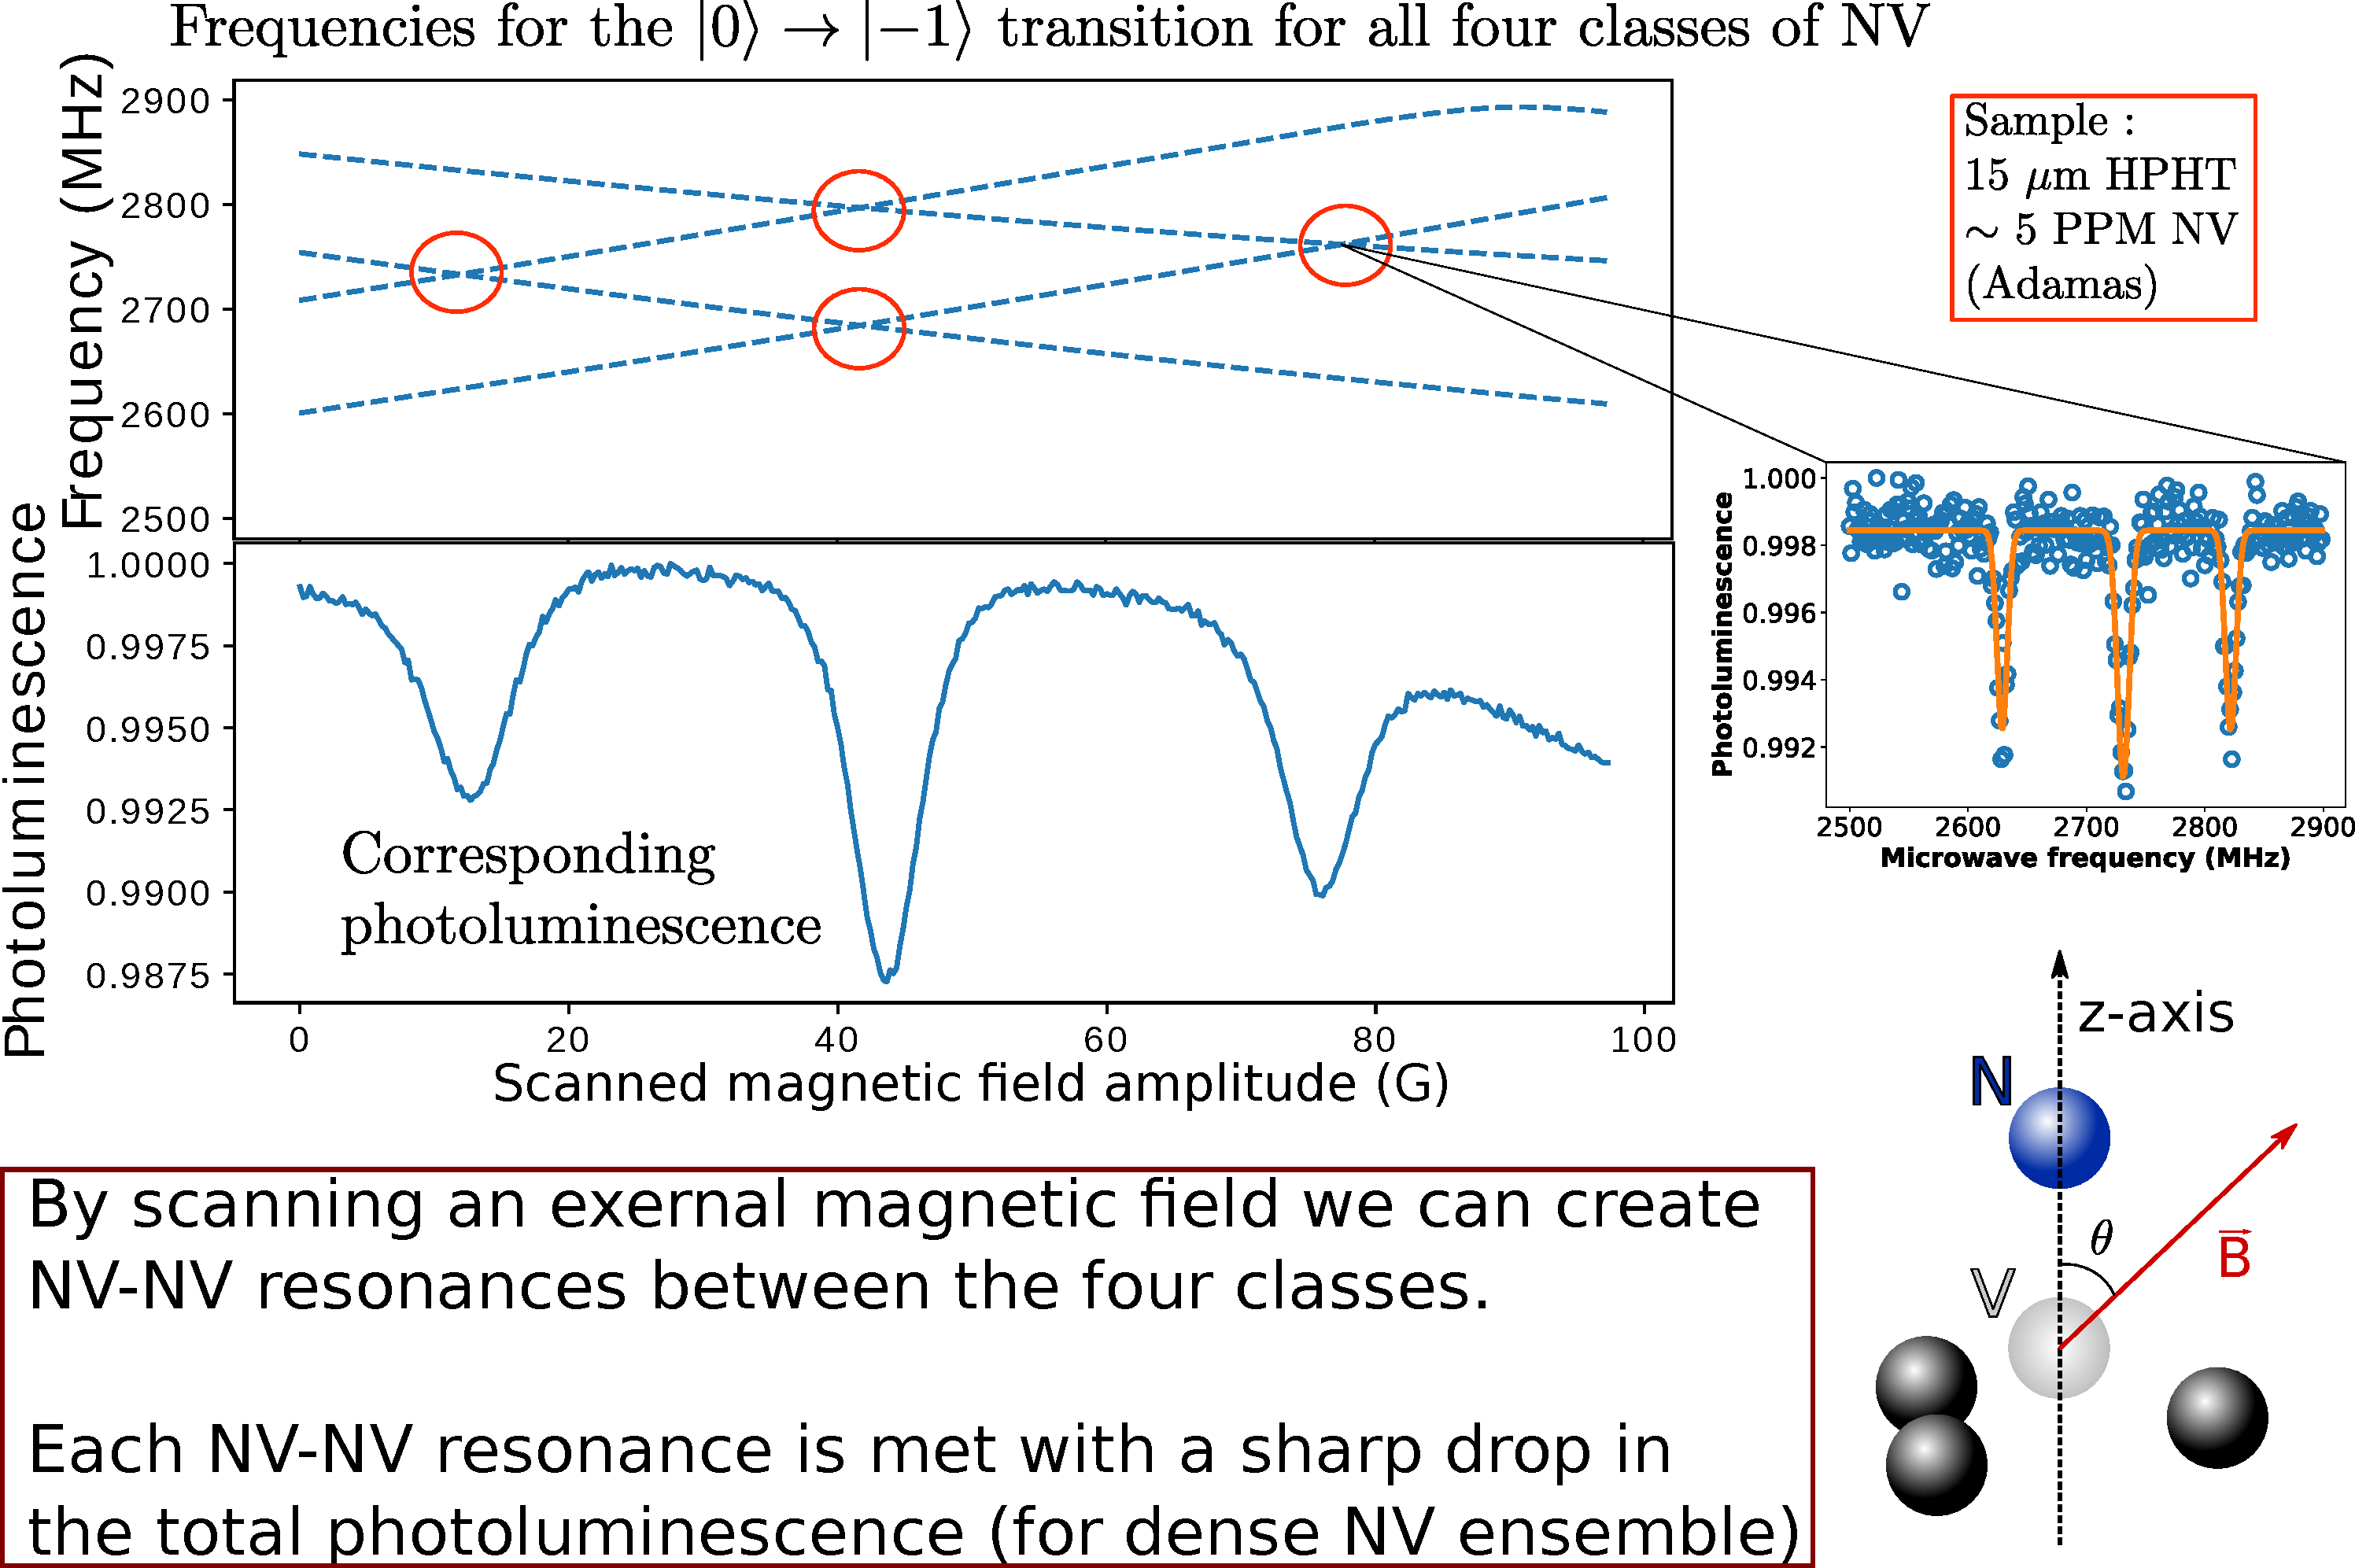
\includegraphics[scale=.2]{Slide_CR_NV-NV}
\end{frame}
\begin{frame}{NV-NV Cross-Relaxation : spin lifetime}
\centering
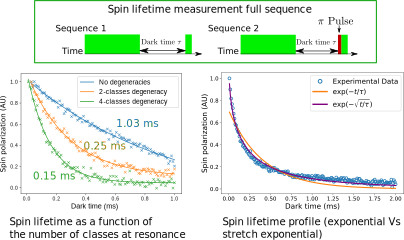
\includegraphics[scale=.28]{Slide_CR_NV-NV_T1}
\end{frame}
\begin{frame}{Origin of the NV-NV cross-relaxation}
Why is it weird ? Because the flip-flop process is spin preserving

$\to$ They should not change the total spin polarization of the NV ensemble.
\bigskip

Hypotheses for the origin of the NV-NV Cross-relaxation :
\begin{itemize}
\item Spin diffusion to unpolarized spins (out of the laser spot)

$\to$ The numbers are off by several order of magnitudes \& it still works with nano-diamond

\item Superradiance $\to$ effect independent of temperature
\item Fluctuators : Some NV have their spin heavily depolarized by tunneling in and out of nearby sites
\item Polarization of the laser ?
\end{itemize}
\end{frame}
\begin{frame}{Mechanically detected Cross-Relaxation}
\centering
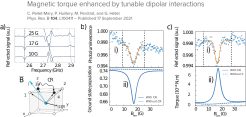
\includegraphics[scale=.45]{slide_cr_meca}
\end{frame}
\section{magnetometry with cross-relaxations}
\begin{frame}
\tableofcontents[currentsection]
\end{frame}
\begin{frame}{Principle of the magnetometer}
\centering
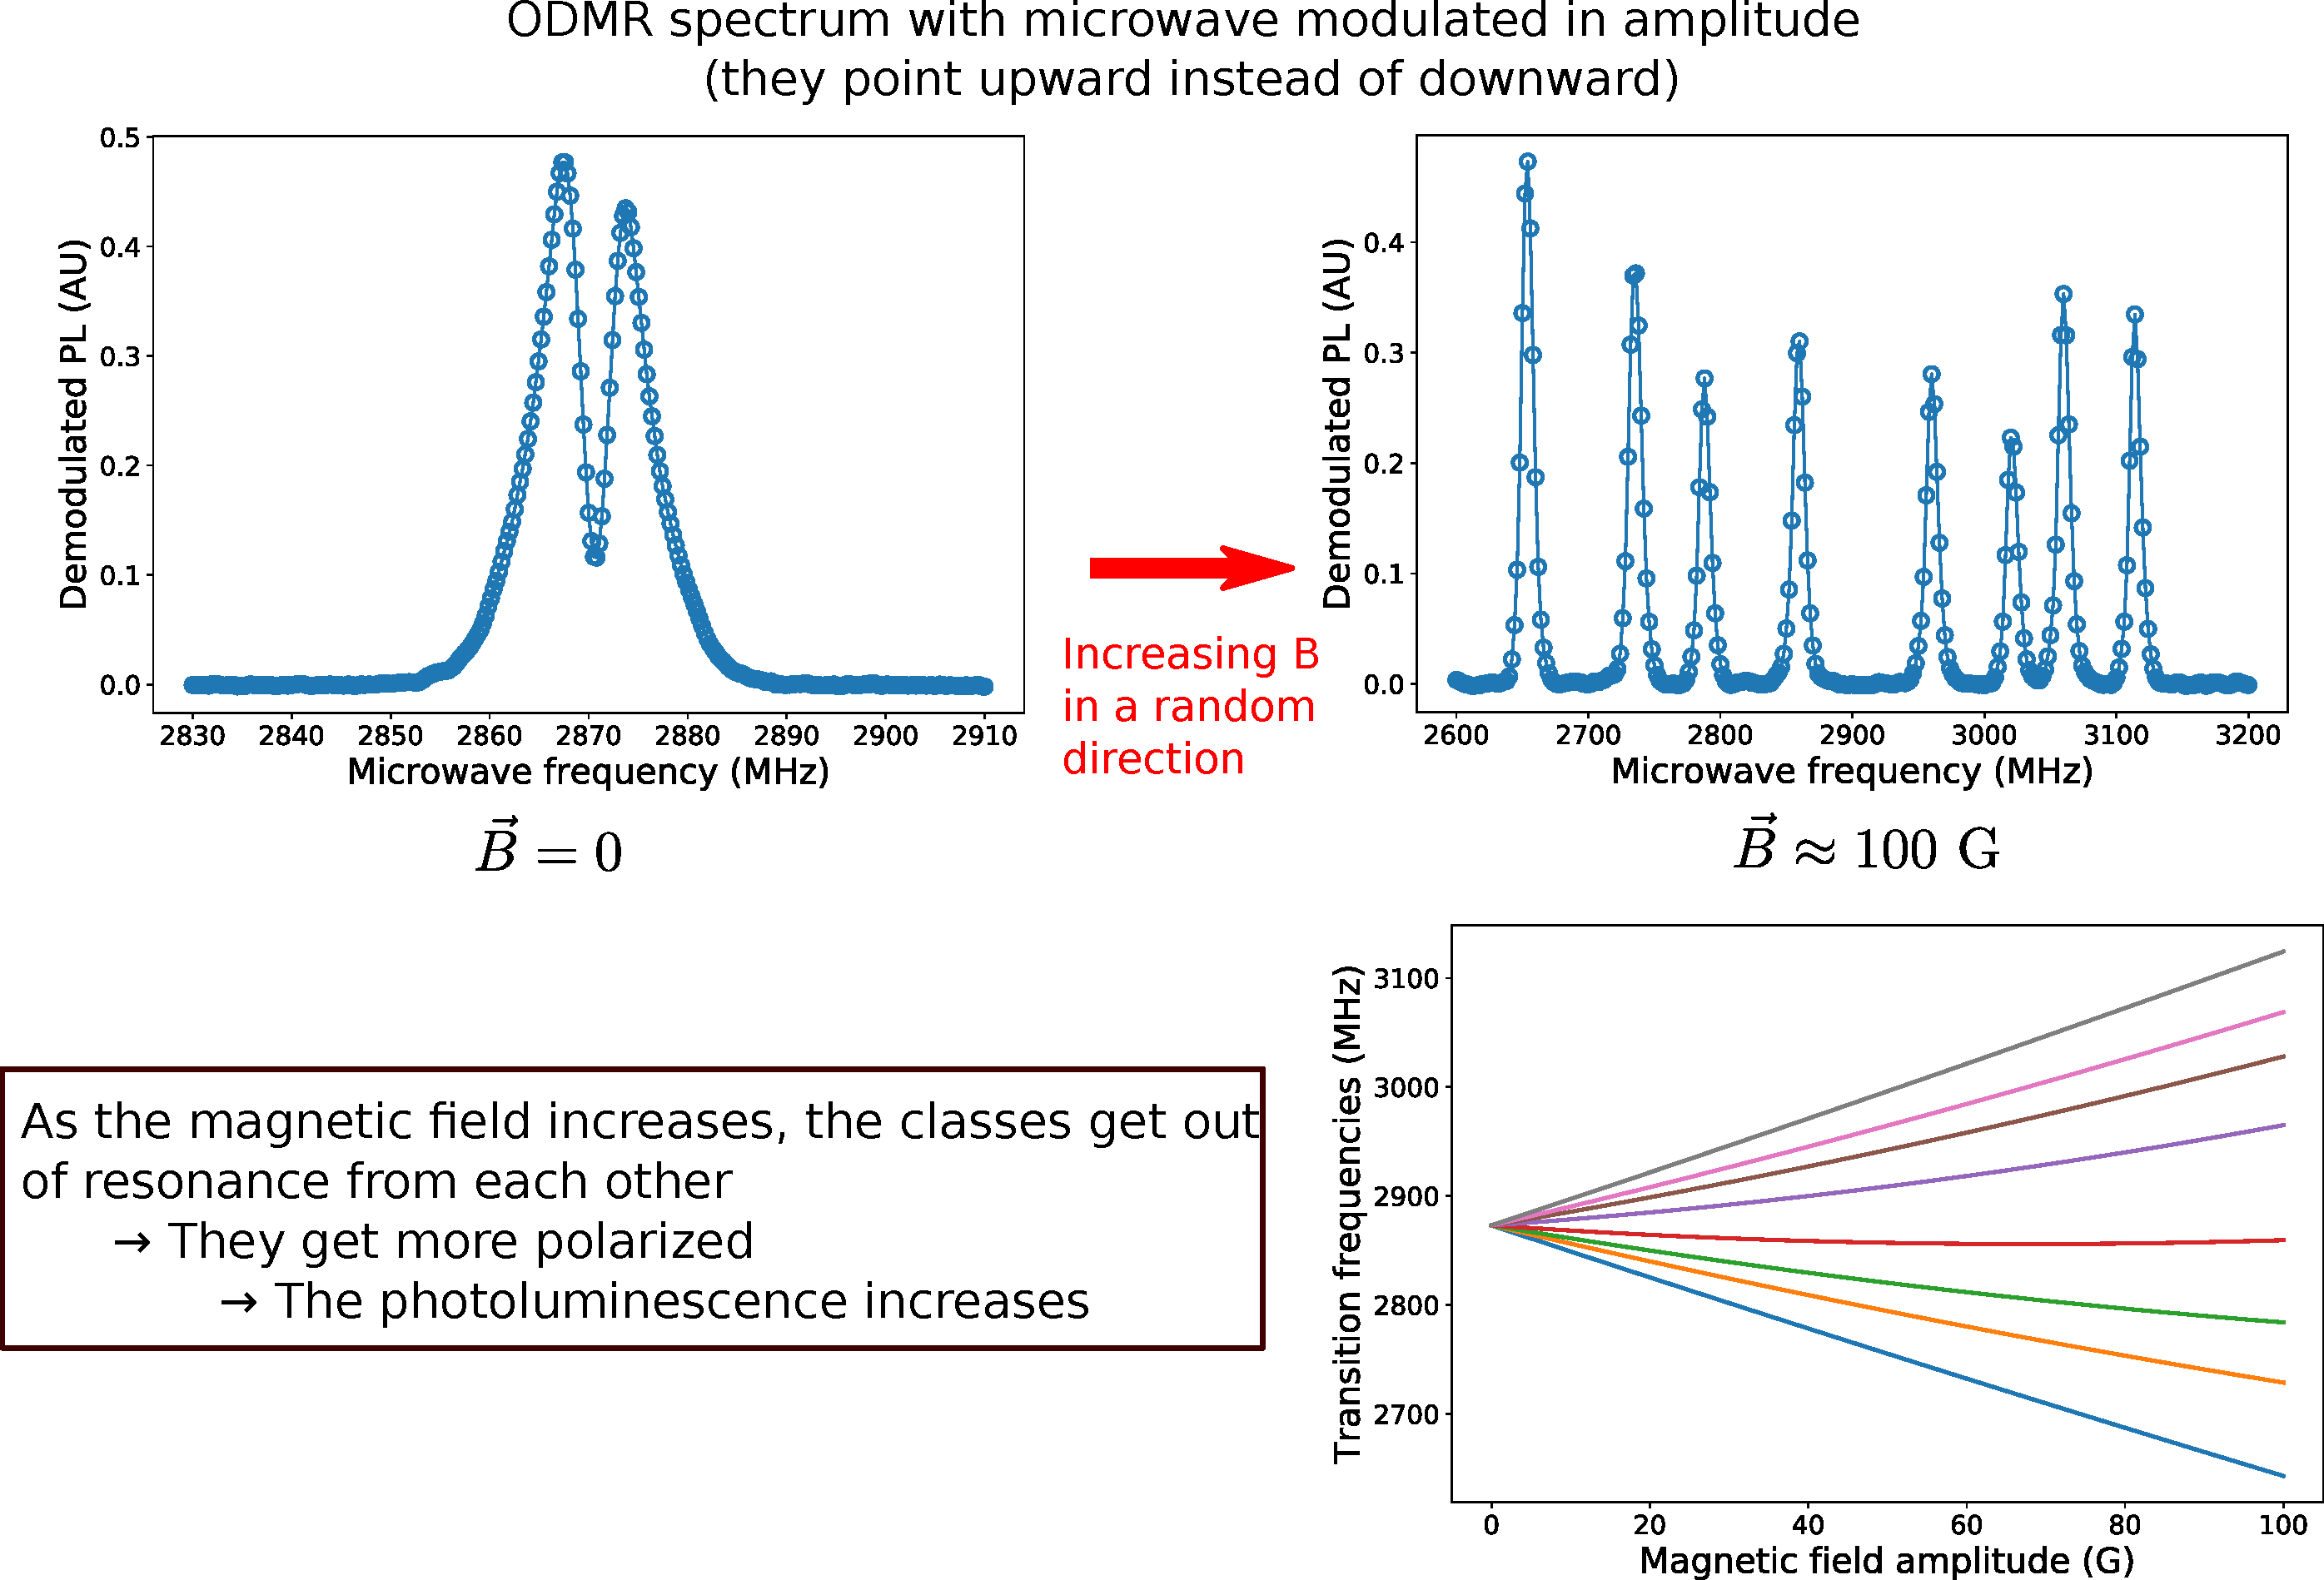
\includegraphics[scale=.22]{Slide_principe_magnetoNVNV}
\end{frame}
\begin{frame}{Low field dependence of the PL}
\centering
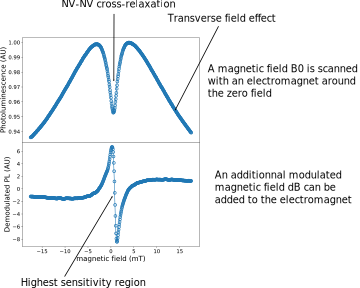
\includegraphics[scale=.23]{slide_magneto_scan}
\end{frame}
\begin{frame}{Sensitivity of the measure}
\centering
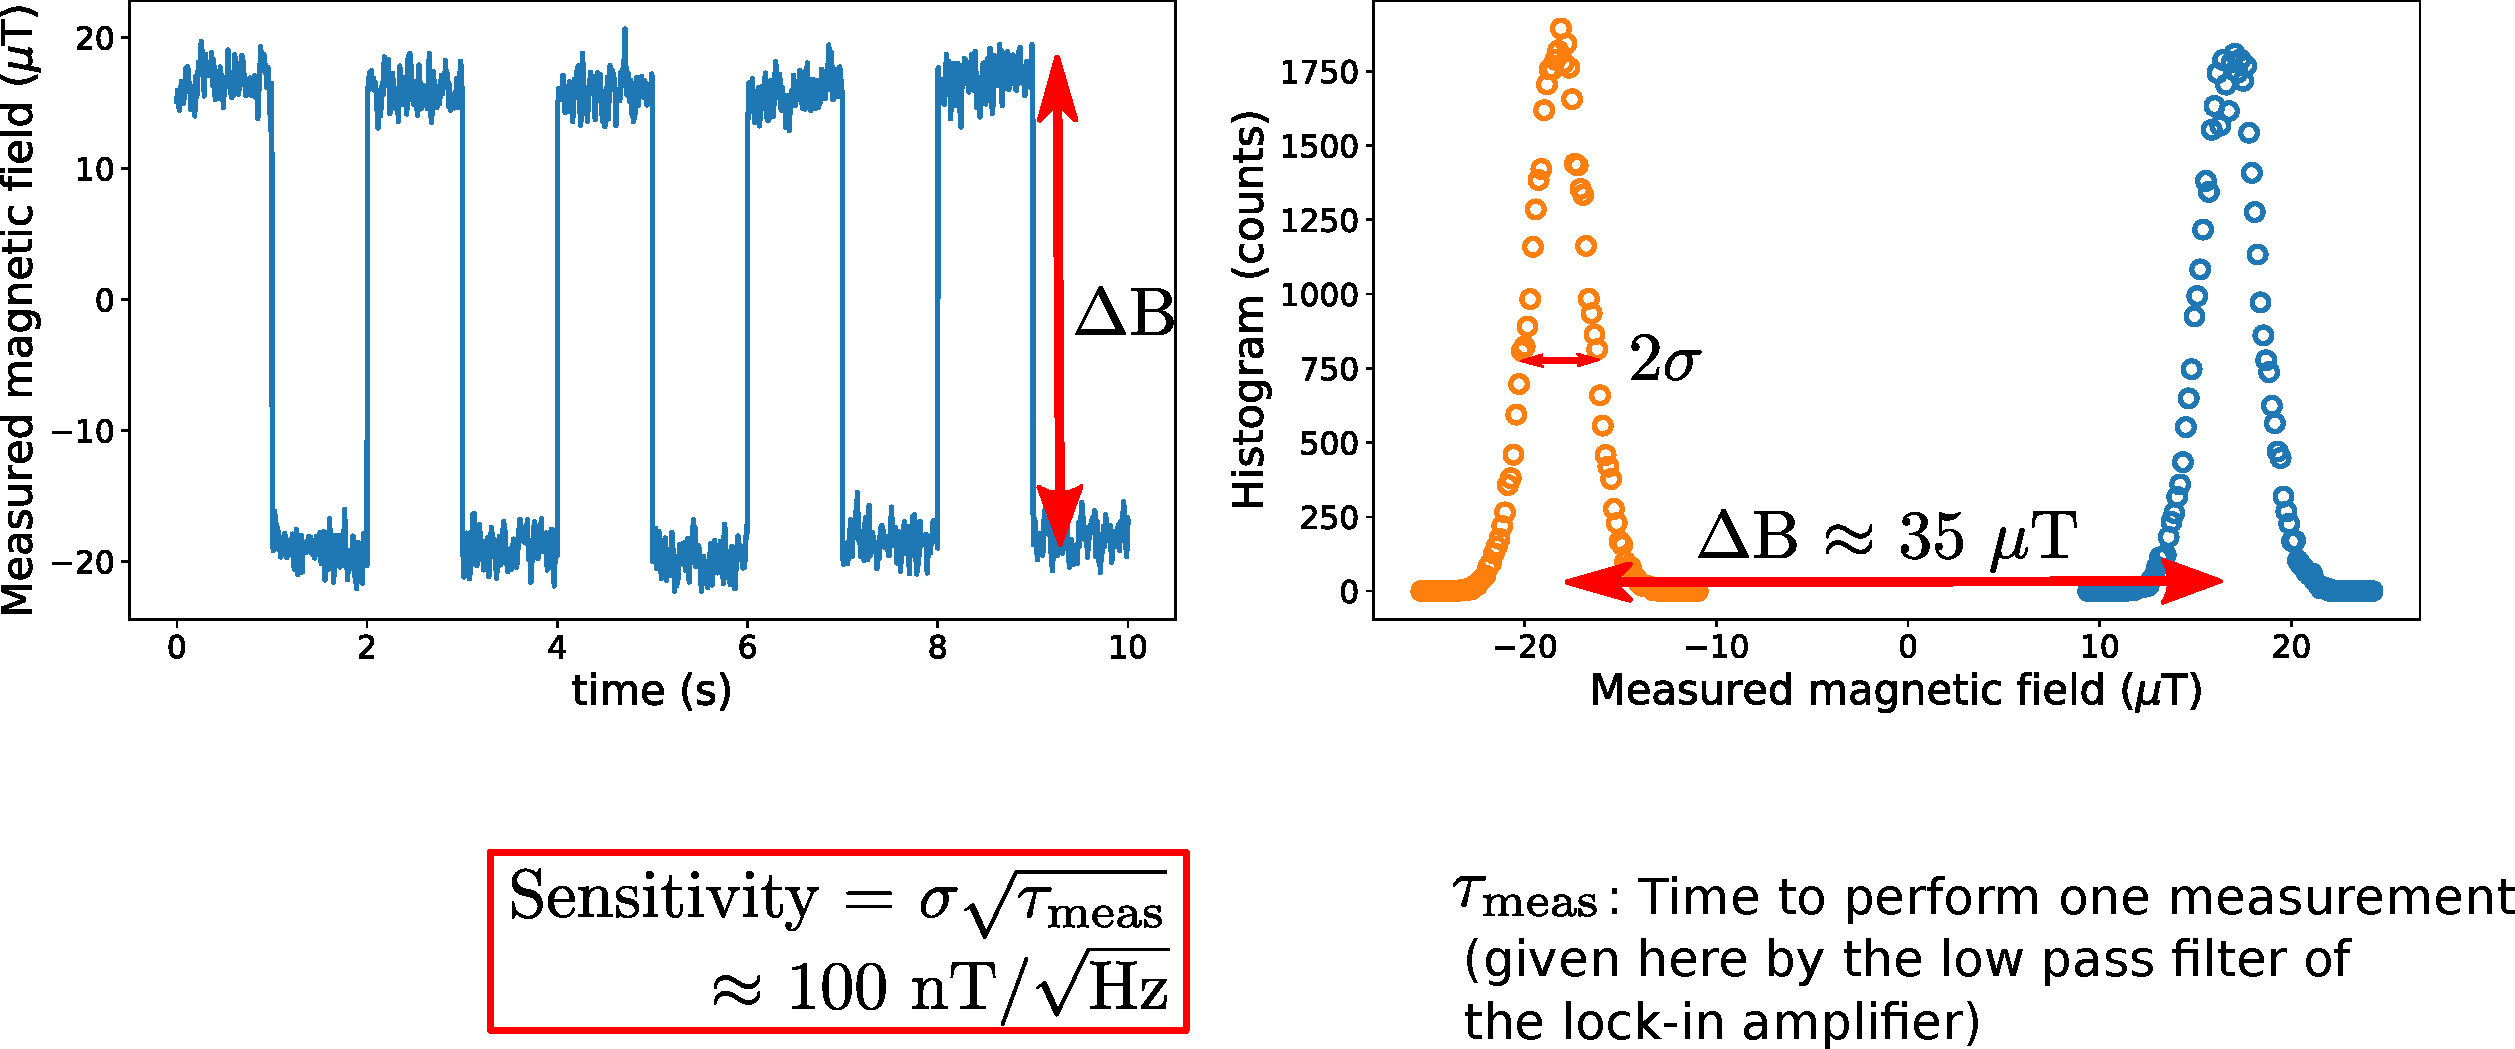
\includegraphics[scale=.26]{slide_sensi_measure}
\end{frame}
\begin{frame}{Comparison with other magnetometer}
\begin{itemize}
\item NV ensemble : $\approx 1$ pT$\sqrt{\textrm{Hz}}$
\item Microwave-less NV ensemble : $\approx 1$ nT$\sqrt{\textrm{Hz}}$
\item SQUIDs(superconducting circuits)/vapor cells : $\approx 1$ fT$\sqrt{\textrm{Hz}}$
\end{itemize}
\bigskip

But,

\begin{itemize}
\item Based on smaller diamonds (10 $\mu$m diamond VS few mm diamonds)
\item Does not require well-defined crystal axis Vs magnetic field orientation

$\to$ Can use poly-crystalline/powdered samples, diamond flow in solution, etc...

\item Better than transverse field by several orders of magnitude
\end{itemize}

\end{frame}
\begin{frame}{Bonus : Double quantum cross-relaxation in zero-field}
\centering
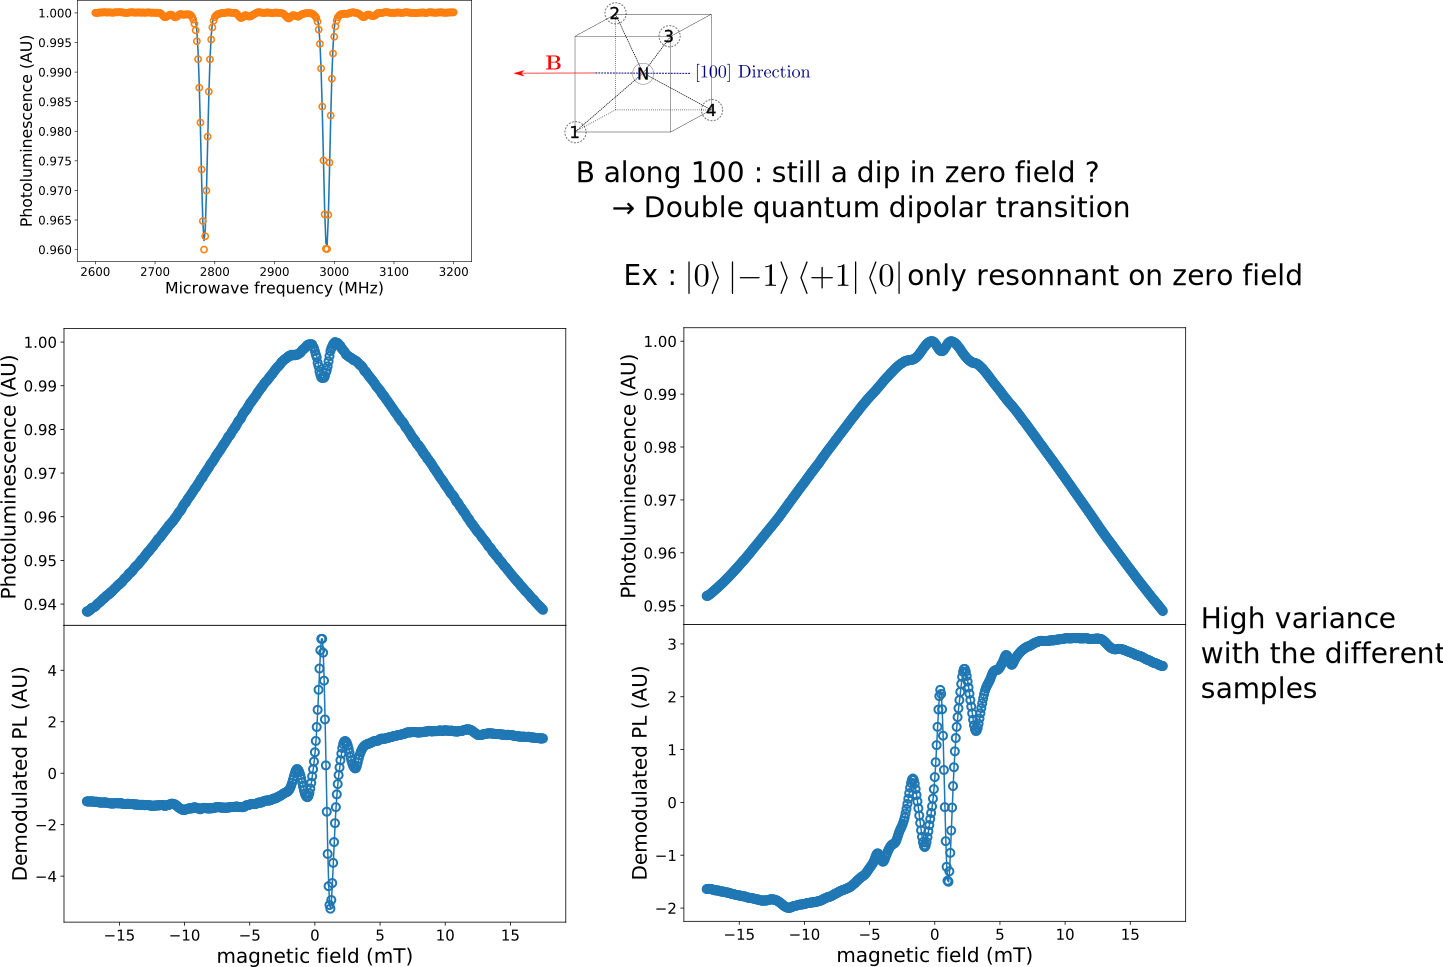
\includegraphics[scale=.22]{slide_DQ}
\end{frame}
\end{document}